\documentclass[]{book}
\usepackage{lmodern}
\usepackage{amssymb,amsmath}
\usepackage{ifxetex,ifluatex}
\usepackage{fixltx2e} % provides \textsubscript
\ifnum 0\ifxetex 1\fi\ifluatex 1\fi=0 % if pdftex
  \usepackage[T1]{fontenc}
  \usepackage[utf8]{inputenc}
\else % if luatex or xelatex
  \ifxetex
    \usepackage{mathspec}
  \else
    \usepackage{fontspec}
  \fi
  \defaultfontfeatures{Ligatures=TeX,Scale=MatchLowercase}
\fi
% use upquote if available, for straight quotes in verbatim environments
\IfFileExists{upquote.sty}{\usepackage{upquote}}{}
% use microtype if available
\IfFileExists{microtype.sty}{%
\usepackage{microtype}
\UseMicrotypeSet[protrusion]{basicmath} % disable protrusion for tt fonts
}{}
\usepackage[margin=1in]{geometry}
\usepackage{hyperref}
\hypersetup{unicode=true,
            pdftitle={RoboCar project documentation},
            pdfauthor={Uwe Sterr},
            pdfborder={0 0 0},
            breaklinks=true}
\urlstyle{same}  % don't use monospace font for urls
\usepackage{natbib}
\bibliographystyle{apalike}
\usepackage{longtable,booktabs}
\usepackage{graphicx,grffile}
\makeatletter
\def\maxwidth{\ifdim\Gin@nat@width>\linewidth\linewidth\else\Gin@nat@width\fi}
\def\maxheight{\ifdim\Gin@nat@height>\textheight\textheight\else\Gin@nat@height\fi}
\makeatother
% Scale images if necessary, so that they will not overflow the page
% margins by default, and it is still possible to overwrite the defaults
% using explicit options in \includegraphics[width, height, ...]{}
\setkeys{Gin}{width=\maxwidth,height=\maxheight,keepaspectratio}
\IfFileExists{parskip.sty}{%
\usepackage{parskip}
}{% else
\setlength{\parindent}{0pt}
\setlength{\parskip}{6pt plus 2pt minus 1pt}
}
\setlength{\emergencystretch}{3em}  % prevent overfull lines
\providecommand{\tightlist}{%
  \setlength{\itemsep}{0pt}\setlength{\parskip}{0pt}}
\setcounter{secnumdepth}{5}
% Redefines (sub)paragraphs to behave more like sections
\ifx\paragraph\undefined\else
\let\oldparagraph\paragraph
\renewcommand{\paragraph}[1]{\oldparagraph{#1}\mbox{}}
\fi
\ifx\subparagraph\undefined\else
\let\oldsubparagraph\subparagraph
\renewcommand{\subparagraph}[1]{\oldsubparagraph{#1}\mbox{}}
\fi

%%% Use protect on footnotes to avoid problems with footnotes in titles
\let\rmarkdownfootnote\footnote%
\def\footnote{\protect\rmarkdownfootnote}

%%% Change title format to be more compact
\usepackage{titling}

% Create subtitle command for use in maketitle
\newcommand{\subtitle}[1]{
  \posttitle{
    \begin{center}\large#1\end{center}
    }
}

\setlength{\droptitle}{-2em}
  \title{RoboCar project documentation}
  \pretitle{\vspace{\droptitle}\centering\huge}
  \posttitle{\par}
  \author{Uwe Sterr}
  \preauthor{\centering\large\emph}
  \postauthor{\par}
  \predate{\centering\large\emph}
  \postdate{\par}
  \date{2018-02-12}

\usepackage{booktabs}

\begin{document}
\maketitle

{
\setcounter{tocdepth}{1}
\tableofcontents
}
\chapter{Project RoboCar}\label{project-robocar}

We want to build autonomous driving model cars which can master a course
without any human intervention

The project was started during one of those cold dark winter evenings on
8th of February 2018 by

\begin{itemize}
\tightlist
\item
  Elias, who carried this idea with him for quite some time already
\item
  Andreas, who as far as I can tell is interested in just about
  everything
\item
  Finn, who probably never thought about this idea before that day but
  was immediately enthusiastic
\item
  Uwe, who was infected with the idea by Elias in autumn 2017
\end{itemize}

We decided then and there to build autonomous robotic cars probably with
Raspberry Pi, but open for all possible concepts.

We organize our meetings via the meetup group
\url{https://www.meetup.com/Esslingen-Makerspace/}, you are welcome to
join in, register as a member of that meetup group and you will receive
invitations to our meetings.

This documentation shall act as an archive for

\begin{itemize}
\tightlist
\item
  Links to resources
\item
  Experiences gathered
\item
  Minutes of meeting
\end{itemize}

\chapter{Resources}\label{resources}

In this section interesting resources for different topics are listed

\section{Meetups}\label{meetups}

\subsection{Esslinger Makerspace Projekt: Autonomen RoboCar
bauen}\label{esslinger-makerspace-projekt-autonomen-robocar-bauen}

\url{https://www.meetup.com/Esslingen-Makerspace/}

Ob ihr euer eigenes RoboCar entwickeln wollt, oder lieber ein kleines
Team bilden wollt, hier seit ihr richtig.

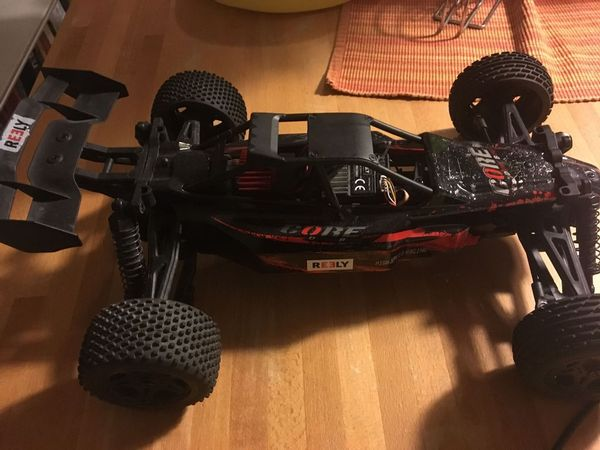
\includegraphics[width=8.33in]{images/EliasCar}

\subsection{Autonomous Mobility
Berlin}\label{autonomous-mobility-berlin}

\url{https://www.meetup.com/autonomous-mobility-berlin/}

This is a group for anyone interested and intrigued by Autonomous
Mobility, Self-Driving Cars (SDC). Robots. We will cover topics on
related technologies - Computer Vision, Deep Learning, Reinforcement
learning, evolutionary computation, Sensor Fusion, ROS etc..

\section{RoboCar projects}\label{robocar-projects}

\subsection{DIY RoboCars}\label{diy-robocars}

\url{https://diyrobocars.com/about/}

This is the sister site to DIY Drones and resource/community companion
to the DIY Robocars Meetup Group. Created by Chris Anderson of 3DR.

\subsection{Donkey car}\label{donkey-car}

\url{http://www.donkeycar.com}

An opensource DIY self driving platform for small scale cars. RC CAR +
Raspberry Pi + Python (tornado, keras, tensorflow, opencv, \ldots{}.)

The \href{http://docs.donkeycar.com}{documentation} of the project
includes:

\begin{enumerate}
\def\labelenumi{\arabic{enumi}.}
\tightlist
\item
  Assemble hardware.
\item
  Install software.
\item
  Calibrate your car.
\item
  Start driving.
\item
  Train an autopilot.
\item
  Experiment with simulator
\end{enumerate}

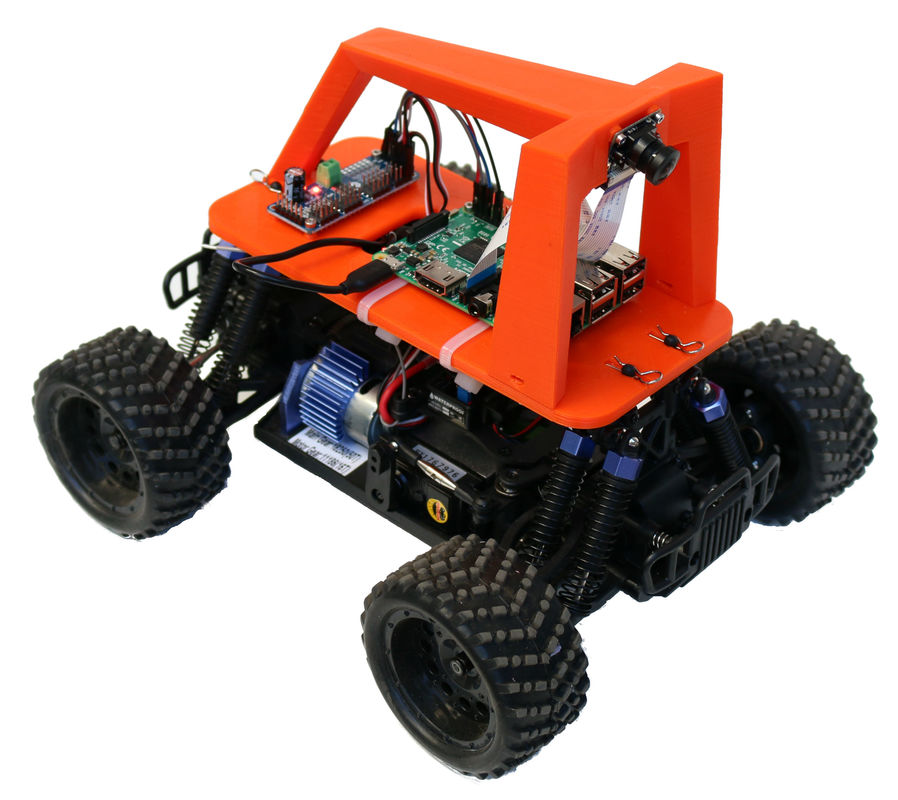
\includegraphics[width=12.47in]{images/donkey-car-graphic_orig}

The code can be found at
\href{https://github.com/wroscoe/donkey}{github}

\subsection{Sunfounder Smart Video Car Kit for Raspberry Pi with Android
App}\label{sunfounder-smart-video-car-kit-for-raspberry-pi-with-android-app}

\url{https://www.sunfounder.com/robotic-drone/smartcar/smart-video-car-kit/rpi-car.html}

This is a complete learning kit based on Raspberry Pi with Android App.
For better learning, an elaborately-written user manual, code with
explanation and thorough schematic diagrams are provided.

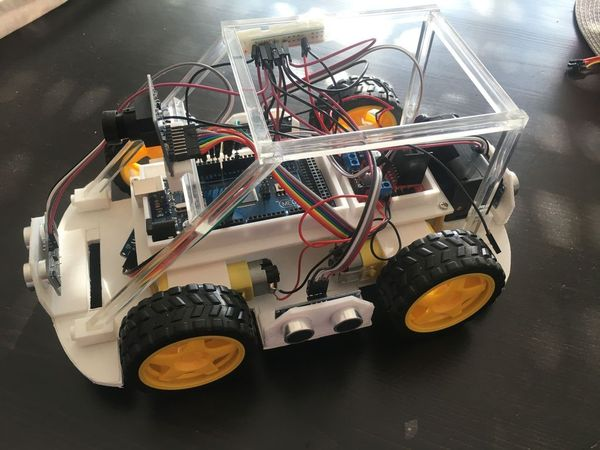
\includegraphics[width=8.33in]{images/sunfounder}

Sunfounder software is found at
\href{https://github.com/sunfounder/Sunfounder_Smart_Video_Car_Kit_for_RaspberryPi}{github}

\section{Simulators}\label{simulators}

\subsection{Donkey Simulator}\label{donkey-simulator}

\url{http://docs.donkeycar.com/guide/simulator/}\\
Experiment with training a donkey car to drive in simulation. This
simulator is built on the the Unity game platform, uses their internal
physics and graphics, and connects to a donkey Python process to use our
trained model to control the simulated Donkey.

\section{Software}\label{software}

\subsection{Udacitiy open source SDC}\label{udacitiy-open-source-sdc}

\url{https://github.com/udacity/self-driving-car}

At Udacity, we believe in democratizing education. How can we provide
opportunity to everyone on the planet? We also believe in teaching
really amazing and useful subject matter. When we decided to build the
Self-Driving Car Nanodegree program, to teach the world to build
autonomous vehicles, we instantly knew we had to tackle our own
self-driving car too.

Together with Google Self-Driving Car founder and Udacity President
Sebastian Thrun, we formed our core Self-Driving Car Team. One of the
first decisions we made? Open source code, written by hundreds of
students from across the globe!

\chapter{Experiences gathered}\label{experiences}

Here I will write down how the adventure goes

\chapter{Minutes of meeting}\label{minutesOfMeeting}

In this section short minutes of meetings are kept so that people who
join later can easily get up to speed

\section{8-02-2018}\label{section}

\subsection{Location: Shackspace}\label{location-shackspace}

What was meant to be a an introduction into the shackspace evolved to a
discussion about various topics

\subsection{Studie Hackerspaces}\label{studie-hackerspaces}

\begin{itemize}
\tightlist
\item
  \url{http://www.cowerk.org/home/single/article/befragungsergebnisse-wertschoepfung-in-offenen-werkstaetten.html}
\item
  \url{https://www.heise.de/make/meldung/Studie-Neue-Produktionsmodelle-in-offenen-Werkstaetten-3504625.html}
\item
  \url{https://www.heise.de/make/meldung/Kein-Freifahrtschein-fuer-Hackerspaces-Benutzung-auf-eigene-Gefahr-3955181.html}
\end{itemize}

\subsection{Buchtipps}\label{buchtipps}

\begin{itemize}
\tightlist
\item
  Makers: Das Internet der Dinge: die nächste industrielle Revolution,
  Chris Anderson
\item
  Zero
\item
  Thinking fast and slow, Kahnemann
\item
  Gunter Dueck
\item
  \url{https://www.omnisophie.com}\\
\item
  Vorträge auf der Re-publica als Einstieg
  \url{https://www.youtube.com/results?search_query=gunter+dueck}
\item
  Biohacking: Gentechnologie für alle, Rüdiger Trojok
\item
  Biohacking: Gentechnik aus der Garage, Hanno Charisius
\end{itemize}

\subsection{RoboCar}\label{robocar}

Elias says he would like to be build an autonomous model car, probably
based on Raspberry Pi. In order to end dreaming and start doing we fixed
the next meeting to 15th of February where we want to start defining
concepts.

\section{15-02-2018}\label{section-1}

\bibliography{book.bib,packages.bib}


\end{document}
